\documentclass[conference]{IEEEtran}
\usepackage{cite}
\usepackage{amsmath,amssymb,amsfonts}
\usepackage{algorithmic}
\usepackage{graphicx}
\usepackage[utf8]{inputenc}
\usepackage[english]{babel}
\usepackage{textcomp}
\usepackage{xcolor}
\def\BibTeX{{\rm B\kern-.05em{\sc i\kern-.025em b}\kern-.08em
    T\kern-.1667em\lower.7ex\hbox{E}\kern-.125emX}}
%\usepackage[
%backend=biber,
%style=alphabetic,
%sorting=ynt
%]{biblatex}

\begin{document}
\raggedright
\title{Multi-Agent control for a Lego PiStorms System}

\author{\IEEEauthorblockN{1\textsuperscript{st} Hendriks Pieter}
\IEEEauthorblockA{\textit{Department of Computer Science} \\
\textit{University of Antwerp}\\
Antwerp, Belgium \\
pieter.hendriks@student.uantwerpen.be}
}
\maketitle

\begin{abstract}

This document describes the implementation of a multi-agent system as a way to control a plastic recycling facility built using Lego parts. The implemented multi-agent system mimics (and slightly extends) the behaviour of the recycling plant built according to the instructions (using Lego EV3 bricks as controllers, with provided code). We replaced the EV3 bricks with Raspberry Pi boards (and the PiStorms attachment) to control the motors and sensors, then ran the multi-agent system on the Raspberry Pis. A few non-essential agents are introduced into the system to extend the functionality.

\end{abstract}

\begin{IEEEkeywords}
Multi-Agent System, Lego, PiStorms, mindsensors, EV3
\end{IEEEkeywords}

\section{Introduction}

This document describes the implementation of a multi-agent system in order to control a Lego plastic recycling plant. The plastic recycling plant comes with EV3 controller bricks, that we have replaced in order to implement the system. The system is now controlled using Raspberry Pi boards, using the PiStorms attachment in order to interface with the Lego sensors and motors. 

Each sensor and motor is controlled by its own agent in the system and three extra agents are present. One for the output on the Raspberry Pis, one for output on a remote computer (think controller station) and one control agent to pass commands into the system (either broadcast or to a specific agent). The control agent allows fine-grained control of the system and, combined with the remote output, is sufficient for the implementation of an automatic plant where human intervention is necessary only when a problem occurs.

\section{Related works}

SPADE \cite{SPADE} is a software framework for the creation of multi-agent systems using an XMPP server to facilitate agent communications. This document provides such an implementation using SPADE. 

In \cite{powerplant}, a multi-agent system is used to control a power plant. Since for a power plant, there are many different parameters to try and optimize, a multi-agent system is a nice way of solving the problem as each agent could try and optimize for a single parameter, where the agents interact in order to approach an optimal overall solution. Our system is less complex, as our plant is rather limited. The flow of problem solving in our case is rather linear, to be expected for an assembly line. 

In \cite{Chemical}, a multi-agent system is used to simulate and support the management of a chemical supply chain. Supply chain management is a complex problem where many issues can arise. Due to the many different actors involved in the supply chain process, a multi-agent system is a very natural approach to solving the problem. This system is implemented using a different communication layer between the agents, but that layer shouldn't have significant impact on the functionality. 


\section{System Design}

The system is controlled using 6 engines and 4 sensors. We'll briefly discuss each of them in order to be able to easily refer to them later on in the paper. The indexing used to identify each motor or sensor mimics that used in the Lego EV3 brick. The first number is the layer the brick is running on (Lego EV3 bricks can be chained in order to provide multiple ports, allowing more complex robots). The second is a number or letter and identifies the port on the brick, this is a number for sensors and a letter for motors. 
\begin{itemize}
\item[1, 1] A touch sensor, that is used in order to start the system. The line operates one brick at a time and this sensor must be pressed in order to work on the next brick whenever the previous one is finished.
\item[1, 2] A color sensor over the in-feed. It detects whether the feed has a brick ready to be dropped. It detects the color after sensor(1, 1) is pressed. It identifies whether a brick is ready to drop onto the assembly line and what color it is.
\item[1, 3] An ultrasonic sensor used to detect if the area around the system is clear when there are many moving parts. This ensures there are no accidents.
\item[1, 4] A second color sensor, later on in the assembly line. This sensor determines which bin the brick should be sorted into. 

\item[1, A] This motor drops bricks onto the assembly line.
\item[1, B] This motor moves the assembly line.
\item[1, C] This motor moves the wash and shred arms over the assembly line.
\item[2, B] This motor ejects the final product from the building position.
\item[2, C] This motor pushes bricks into the sorting bins when they are not the currently configured building color.
\item[2, D] This motor handles the building process when correctly coloured bricks arrive at the building position. 
\end{itemize}

A happy-path run of the system would then be as follows: sensor(1, 1) touched, sensor(1, 2) detects correct color, motor(1, A) drops brick onto line, motor(1, B) moves brick forward, motor(1, C) shreds and cleans, sensor(1, 3) verifies nothing in close proximity, sensor(1, 4) detects the brick is the color we want to build with, motor(2, C) remains still because the brick must remain on the assembly line, the brick arrives in the building position at the end of the line, motor(2, D) uses it to build and then motor(2, B) ejects the final product. 
Any time a sensor is involved, one (or more) alternative paths occur depending on the value the sensor scans. Based on those values, the system stops moving (if proximity is detected), requires human intervention (if sensor(1, 4) detects a bad color, sorts into one of the bins (if sensor(1, 4) detects one of the three other colors). The assembly line will also reverse in order to attempt to fix a brick that has gotten stuck if the assembly line motor detects that the brick should have arrived, but the system hasn't handled it yet.

\subsection{Multi-agent system design}

Before, we generically described the system and how it functions out of the box. Now, we'll discuss how we translated that behaviour into a multi-agent system. Step one, of course, is determining what the system use cases actually are. In figure \ref{requirements} we clearly model what the requirements the system must fulfil are. These simply mimic the description of the system we gave above.

\begin{figure}[htbp]
\centerline{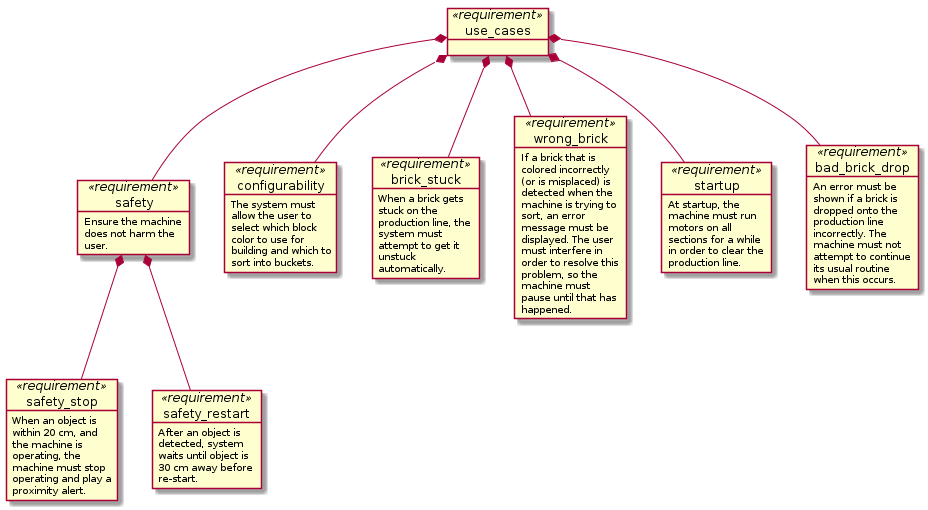
\includegraphics[width=0.45\textwidth]{sysml/requirements.png}}
\caption{The SysML\cite{sysml} model of our use-case requirements}
\label{requirements}
\end{figure}


\subsubsection{Agents} 

Clearly, an important part of a multi-agent system is what to actually model as agents. Generally, when picking agents, one looks at what the actors in the system are and then each actor in the system is modelled as an agent. In this case, there were two ways of doing that. Either every sensor and motor is its own agent, or each controller is an agent. Due to the fact that there is no clear separation between the function of the two controllers, the former option seemed more intuitive for this implementation.

In the case the controllers each controlled their own section of the assembly line, without any overlap, that choice would have been more attractive for simplicity. In this case, though, there is overlap which makes it a somewhat less intuitive model. 

\begin{figure}[htbp]
\centerline{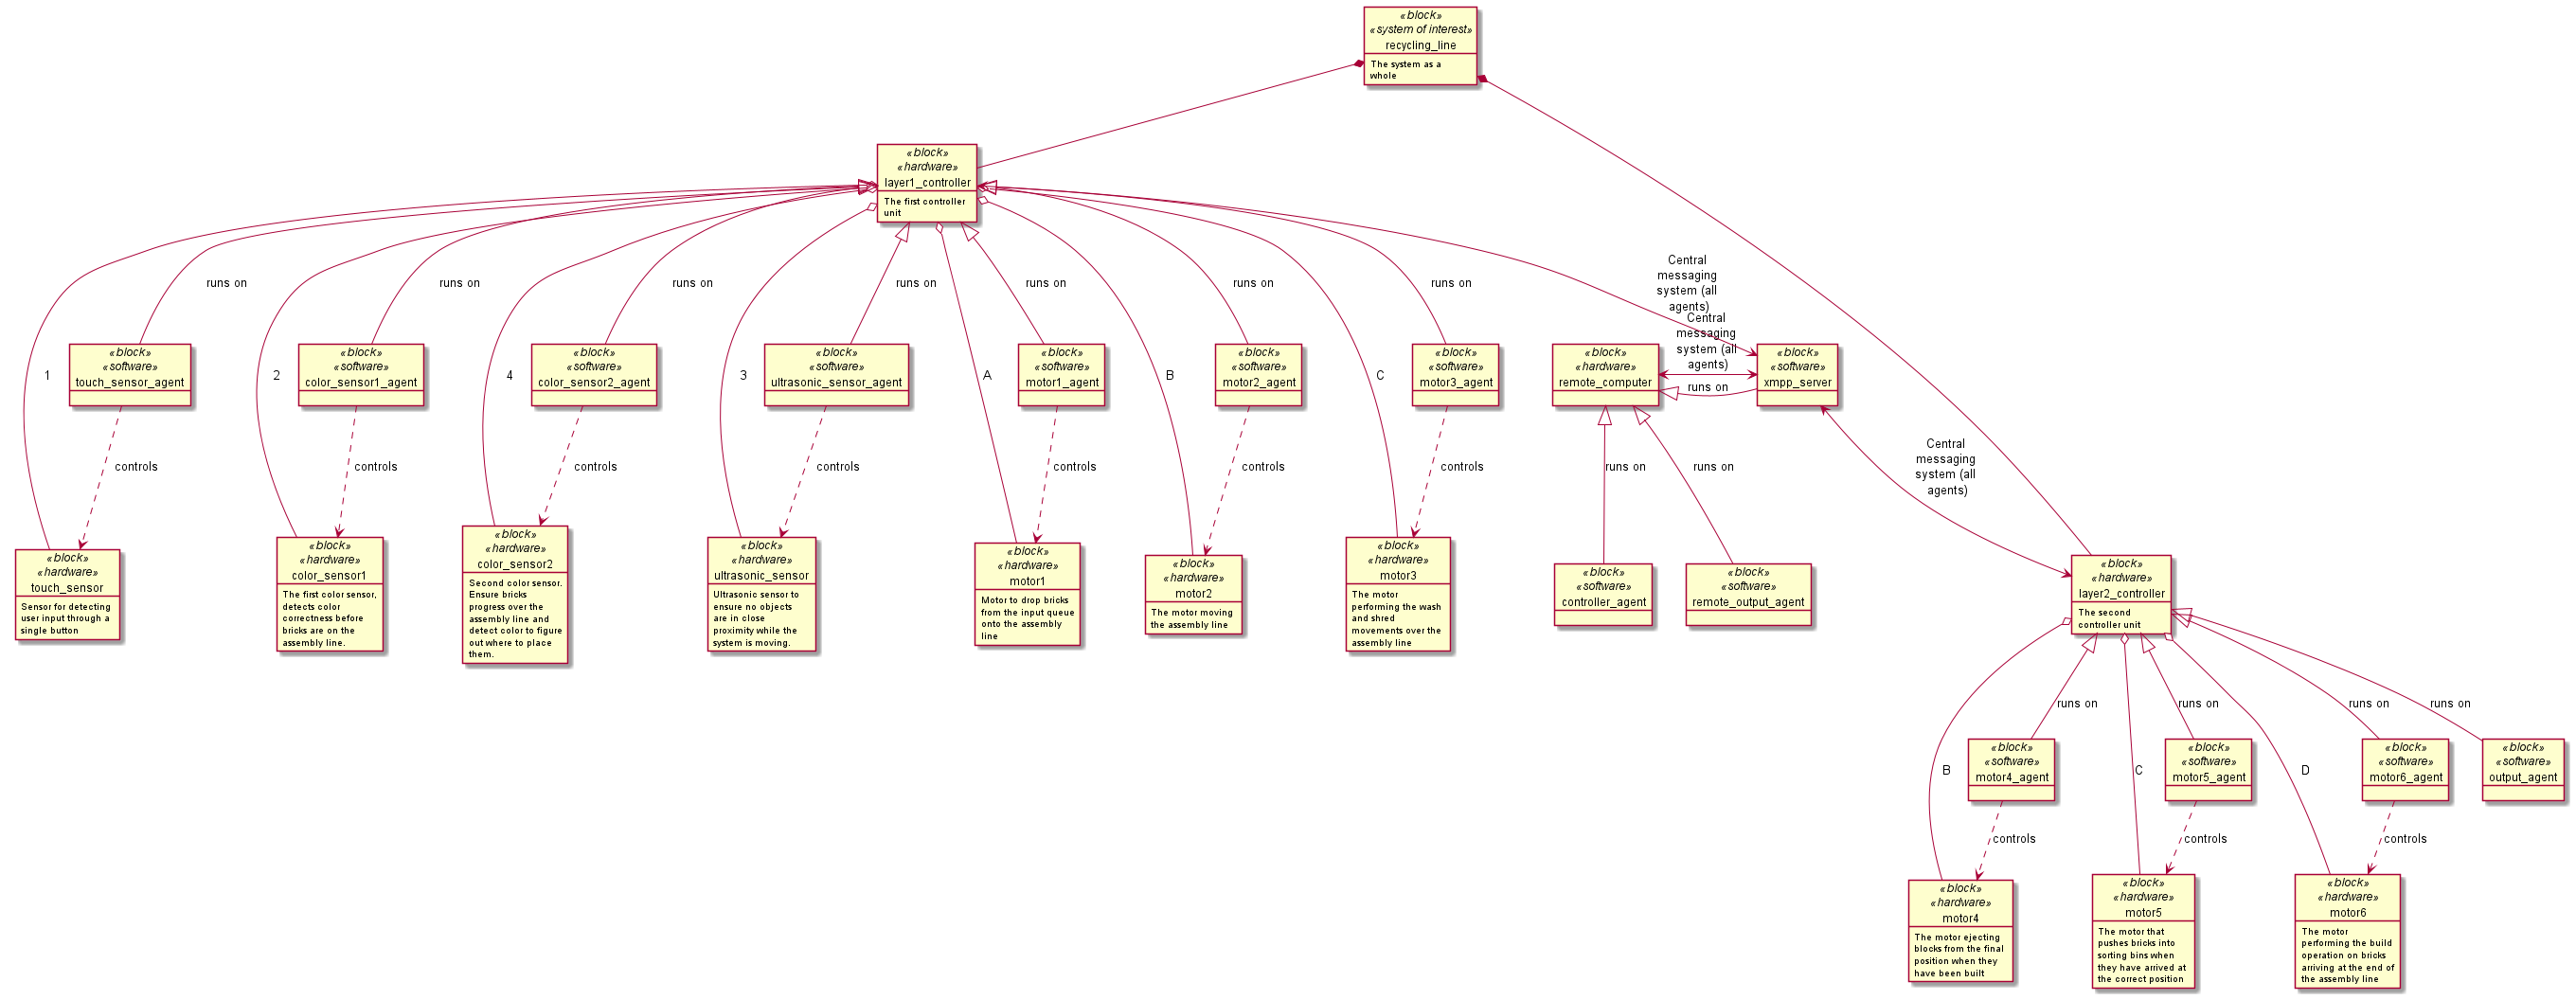
\includegraphics[width=0.45\textwidth]{sysml/architecture.png}}
\caption{The SysML\cite{sysml} model of our multi-agent system architecture}
\label{architecture}
\end{figure}

In figure \ref{architecture} we model, in detail, what the function of each agent is and what hardware they run on. This will not be further addressed in the text - knowing each motor and sensor is controlled by its own agent should be sufficient. 

\subsubsection{Communication}

The communication between the agents is how a multi-agent system is able to actually solve any task. The communication is handled using an XMPP server, as implemented in SPADE \cite{SPADE}. For our case, a local XMPP server was used with each agent having its own account on the server. Account names and server location are in a separate file for easy configuration. 

The messages exchanged between the agents will be shown using another SysML\cite{sysml} diagram, figure \ref{comms}. The figure doesn't fully cover every message that can be exchanged, some have been omitted for readability. The general idea should be clear from this image, though. 

\begin{figure}[htbp]
\centerline{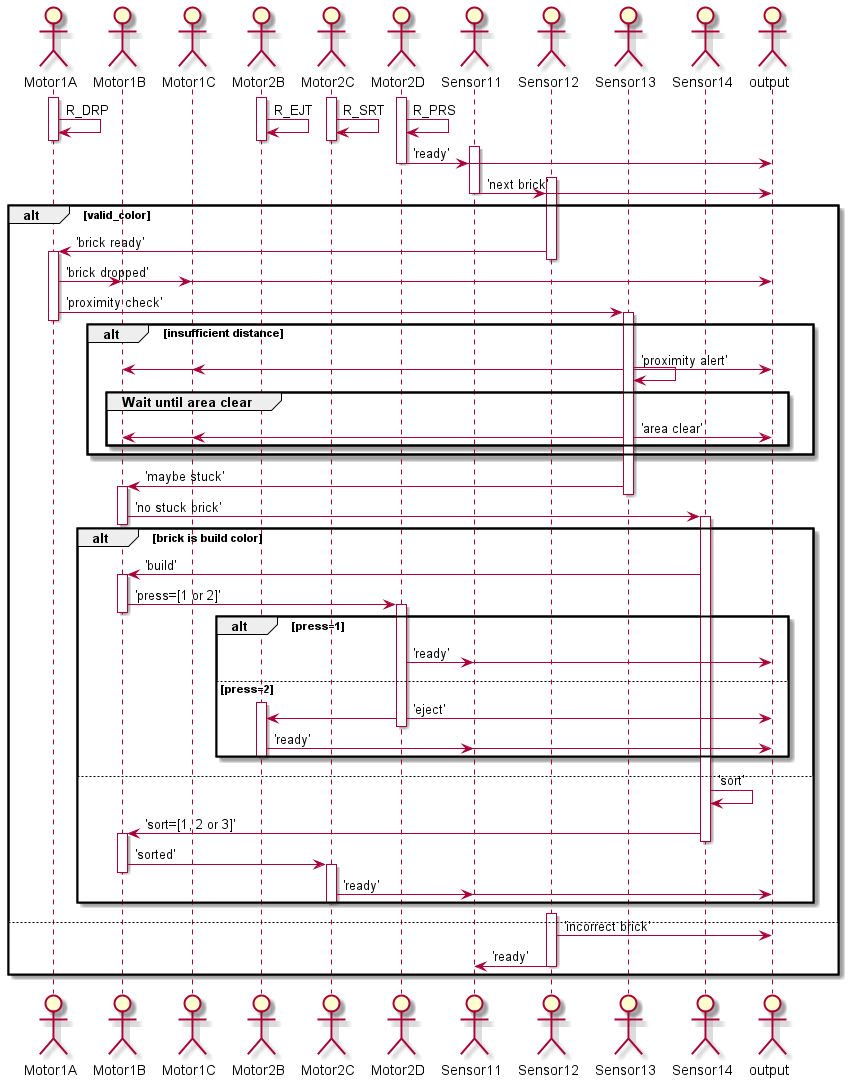
\includegraphics[width=0.45\textwidth]{sysml/communications.png}}
\caption{The SysML\cite{sysml} model of the agent message exchange}
\label{comms}
\end{figure}

\subsubsection{Remote Control}

As an extension to the functionality of the lego system, we allow a user to interact with a remote computer in order to control the system. This functionality is somewhat split over two agents - one handling the display of information received from the agents (can also be used for e.g. error handling, logging, ...). The other takes the user input and passes it on to the agents. The front end for this control use is very rough and rather unwieldy, but serves as a sufficient proof of concept. The functionality is illustrated in figure \ref{control}. 

\begin{figure}[htbp]
\centerline{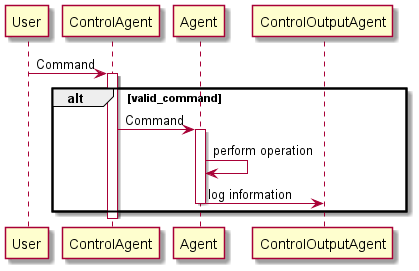
\includegraphics[width=0.45\textwidth]{sysml/control.png}}
\caption{The SysML\cite{sysml} model for the remote control messaging}
\label{control}
\end{figure}

\section{Implementation}

The system is implemented in Python 3.7, running on the Raspberry Pis with a PiStorms attachment. The Python API for the PiStorms is provided by mindsensors, but is mostly only compatible with Python 2. 

SPADE is used to implement the multi-agent system and the Mindsensors PiStorms API is used to interact with the Lego sensors and motors. The system functionality is mostly a direct translation from the Lego Scratch code provided with the Lego building instructions for the recycling plant, but throughout the implementation, small changes have been made. Generally either for ease of development, simplicity of messaging (e.g. sensor sends message to motors A and B instead of only to A, followed by A sending to B after A has finished), or to handle an issue that occurred when doing it the normal way. 

\subsection{Parallelization}

We used Python's multiprocessing module in order to run each agent in its own process. This was done to force all inter-agent communication through the XMPP server. That generalizes the results we obtain, as needing to run agents on the same hardware in some cases could prove to be a problem for a different implementation.

It also ensures the running of one agent has minimal impact on the running of another. 

\subsection{Challenges}

During the development of this system, we faced a few challenges. Some of them were rather easy to correct (or avoid), others posed some longer lasting problems and had more influence on the final result. We discuss a few of the most important ones below.

\subsubsection{Incorrect sensor values}
One of the main problems was that the values sensors record when the measuring function (in the mindsensors API is called) doesn't consistently match the value they should actually be measuring. This also applies to the motors, when reading their rotation. In our implementation, we mostly avoided this (though not fully) by performing several, sequential measurement and taking either the average or the mode (depending on sensor type) of the results in order to determine what the result should be. 

This implementation works for the most part, though occasionally, errors will still pop up. This is definitely a very hacky fix and there must be a prettier way of handling things (presumably through improvement of the API). But given the limited documentation for interaction directly with the hardware, that did not seem like feasible implementation so this was chosen instead. 

\subsubsection{Missing functionality in API}
The mindsensors API as provided did not include a way for us to reset the rotation for a motor. This is a function that is required in order to correctly turn the motors in this system though, so this posed a bit of a problem. An initial solution was to simply implement this functionality on the agent side. We'd record the current rotation in a variable whenever the function is called, then subtract that value from the actual rotation whenever the rotation is read.

That worked for a time, but this later caused a few instances where one of the motors would seem to run infinitely (either because of an overflow somewhere or because of a value being read incorrectly). 

We then modified the API a little bit - an old function \emph{resPos()} was mentioned in the files, but commented out. We re-implemented it, using the implementation of the \emph{pos()} function to determine what a sensible implementation of this function would be. In order to correctly implement it, we also needed to add a few extra implementations further in the backend, directly writing the memory. For these, similar functions were also available and used as examples in order to implement correctly.

\subsubsection{Simultaneity}

While the SPADE API, combined with the Python3 async/await syntax provides some level of simultaneity, it is important to realise that during any synchronous call, the function cannot be interrupted (i.e., an asynchronous function calling e.g. \emph{time.sleep(5)} cannot be interrupted as\emph{time.sleep(5)} is a synchronous call). This means that one of the agent's behaviours waiting would also block the other behaviours on that agent, which turned out to be a problem in a few cases.

An implementation of an asynchronous waiting function corrected this. 

\subsubsection{Remote control}

Since the implementation is a recycling plant, having to manually interact with the system in order to configure e.g. the color of brick to build with, or to start dropping the next brick is suboptimal. We implemented a remote-control agent that allows anyone in a control room (away from the machinery) to interact with the system in a very precise manner. 

The control agent allows arbitrary function execution (e.g. run a certain motor for 5 seconds). It also allows the user to force a sensor the return a certain value (e.g. make a color sensor return the value for red next time it is polled). This allows the user to manipulate what happens to the brick on the assembly line very precisely. 

Of course, the front-end is unwieldy currently, making this infeasible. However, a more elegant implementation could definitely improve that sufficiently to make precise control from a remote computer feasible. 

\section{Conclusion}

The system works as expected, for the most part. Blocks correctly move through the assembly line and are sorted or built with depending on their color (and the current color configuration). 

Since the system is a hardware implementation and easiest to assess visually, the results are shown in a few videos. The videos can be obtained through contact with the author. They are also temporarily available through the link, reference \cite{resultslink}. 

A multi-agent system provides a very natural framework to reason about the implementation of the plastic recycling line. With very limited messaging between the agents (short, keyword messages), essential information can be trivially exchanged while each agent remains fully responsible for its own functions and the cooperation between the agents very elegantly allows a full system to solve the problem it was designed to.

\section{Future work}

Any one agent can be replaced by a different implementation and, based on different messaging sequences, can modify the behaviour of the overall system. This agent-as-a-black-box idea is very interesting because it means the agent complexity can be arbitrarily modified and extended for any agent without impacting any of the others. 

For a more complex system, where the agents have to perform complex computations, that allows the implementation of e.g. a machine learning algorithm for one agent without disturbing the behaviour of any other. 

For our implementation, this could be interesting in the case of the color sensors, for example. Let's say the bricks entering the plant are dirty (as implied by the motor(1, C)'s washing function). Sufficiently dirty bricks might be hard to identify - a classification algorithm might be used to determine if a given object (seen through a camera - e.g. in sensor(1, 2)'s space) is a brick we want to use or simply a piece of trash.

Many such examples for improvements can be made. For the implementation of a toy-system (such as ours), these mostly are irrelevant. For a real-life use case, though, the potential to improve the system arbitrarily with minimal overhead is a definite plus. 


\begin{thebibliography}{03}
\bibitem{powerplant} J. S. Heo and K. Y. Lee, 'A Multiagent-System-Based Intelligent Reference Governor for Multiobjective Optimal Power Plant Operation', IEEE Transactions on Energy Conversion, vol. 23, pp. 1082-1092, December 2008
\bibitem{SPADE} Gregori, Miguel Escriv\'{a} and C\'{a}mara, Javier Palanca and Bada, Gustavo Aranda, 'A Jabber-Based Multi-Agent System Platform', Hakodate, Japan, 2006, accessed on Dec. 31, 2020. [Online]. Available: https://doi.org/10.1145/1160633.1160866
\bibitem{Chemical} Garc{\'i}a-Flores, Rodolfo and Wang, Xue Zhong, 'A multi-agent system for chemical supply chain simulation and management support', OR Spectrum, vol. 24, pp. 343-370, August 2002
\bibitem{sysml} 'Systems modeling language (SysML) specification', SysML Merge Team, OMG Document,  2006
\bibitem{resultslink} https://drive.google.com/drive/folders/\\ 1sWRTfZLV0R6V5hY9jWtV0HNJnITV4ELS?usp=sharing

\end{thebibliography}
\end{document}
